% Options for packages loaded elsewhere
\PassOptionsToPackage{unicode}{hyperref}
\PassOptionsToPackage{hyphens}{url}
%
\documentclass[
]{book}
\usepackage{amsmath,amssymb}
\usepackage{lmodern}
\usepackage{iftex}
\ifPDFTeX
  \usepackage[T1]{fontenc}
  \usepackage[utf8]{inputenc}
  \usepackage{textcomp} % provide euro and other symbols
\else % if luatex or xetex
  \usepackage{unicode-math}
  \defaultfontfeatures{Scale=MatchLowercase}
  \defaultfontfeatures[\rmfamily]{Ligatures=TeX,Scale=1}
\fi
% Use upquote if available, for straight quotes in verbatim environments
\IfFileExists{upquote.sty}{\usepackage{upquote}}{}
\IfFileExists{microtype.sty}{% use microtype if available
  \usepackage[]{microtype}
  \UseMicrotypeSet[protrusion]{basicmath} % disable protrusion for tt fonts
}{}
\makeatletter
\@ifundefined{KOMAClassName}{% if non-KOMA class
  \IfFileExists{parskip.sty}{%
    \usepackage{parskip}
  }{% else
    \setlength{\parindent}{0pt}
    \setlength{\parskip}{6pt plus 2pt minus 1pt}}
}{% if KOMA class
  \KOMAoptions{parskip=half}}
\makeatother
\usepackage{xcolor}
\usepackage{longtable,booktabs,array}
\usepackage{calc} % for calculating minipage widths
% Correct order of tables after \paragraph or \subparagraph
\usepackage{etoolbox}
\makeatletter
\patchcmd\longtable{\par}{\if@noskipsec\mbox{}\fi\par}{}{}
\makeatother
% Allow footnotes in longtable head/foot
\IfFileExists{footnotehyper.sty}{\usepackage{footnotehyper}}{\usepackage{footnote}}
\makesavenoteenv{longtable}
\usepackage{graphicx}
\makeatletter
\def\maxwidth{\ifdim\Gin@nat@width>\linewidth\linewidth\else\Gin@nat@width\fi}
\def\maxheight{\ifdim\Gin@nat@height>\textheight\textheight\else\Gin@nat@height\fi}
\makeatother
% Scale images if necessary, so that they will not overflow the page
% margins by default, and it is still possible to overwrite the defaults
% using explicit options in \includegraphics[width, height, ...]{}
\setkeys{Gin}{width=\maxwidth,height=\maxheight,keepaspectratio}
% Set default figure placement to htbp
\makeatletter
\def\fps@figure{htbp}
\makeatother
\setlength{\emergencystretch}{3em} % prevent overfull lines
\providecommand{\tightlist}{%
  \setlength{\itemsep}{0pt}\setlength{\parskip}{0pt}}
\setcounter{secnumdepth}{5}
\usepackage{booktabs}
\usepackage{amsthm}
\makeatletter
\def\thm@space@setup{%
  \thm@preskip=8pt plus 2pt minus 4pt
  \thm@postskip=\thm@preskip
}
\makeatother

\usepackage{tcolorbox}


\newtcolorbox{blackbox}{
  colback=black,
  coltext=white,
  colframe=black,
  boxsep=5pt,
  arc=4pt}
\newtcolorbox{bonus}{
  colback=blue!15,
  colframe=blue!15,
  coltext=black!80,
  boxsep=5pt,
  arc=4pt}
\newtcolorbox{reflect}{
  colback=green!5,
  colframe=green!5,
  coltext=black!80,
  boxsep=5pt,
  arc=4pt}
\newtcolorbox{assessment}{
  colback=blue!5,
  colframe=blue!5,
  coltext=black!80,
  boxsep=5pt,
  arc=4pt}
\newtcolorbox{progress}{
  colback=purple!10,
  colframe=purple!10,
  coltext=black!80,
  boxsep=5pt,
  arc=4pt}
\newtcolorbox{video}{
  colback=yellow!5,
  colframe=yellow!5,
  coltext=black!80,
  boxsep=5pt,
  arc=4pt}
\newtcolorbox{caution}{
  colback=red!5,
  colframe=red!5,
  coltext=black!80,
  boxsep=5pt,
  arc=4pt}
\newtcolorbox{feedback}{
  colback=black!5,
  colframe=black!5,
  coltext=black!80,
  boxsep=5pt,
  arc=4pt}
\ifLuaTeX
  \usepackage{selnolig}  % disable illegal ligatures
\fi
\usepackage[]{natbib}
\bibliographystyle{apalike}
\IfFileExists{bookmark.sty}{\usepackage{bookmark}}{\usepackage{hyperref}}
\IfFileExists{xurl.sty}{\usepackage{xurl}}{} % add URL line breaks if available
\urlstyle{same} % disable monospaced font for URLs
\hypersetup{
  pdftitle={{[}Course Name \& \#{]}},
  pdfauthor={Name},
  hidelinks,
  pdfcreator={LaTeX via pandoc}}

\title{{[}Course Name \& \#{]}}
\author{Name}
\date{2023-03-14}

\begin{document}
\maketitle

{
\setcounter{tocdepth}{1}
\tableofcontents
}
\hypertarget{course-description}{%
\chapter*{Course Description}\label{course-description}}
\addcontentsline{toc}{chapter}{Course Description}

\emph{Insert the course description here.}

\begin{feedback}
\textbf{Tips for Instructors:} Consider this description as a hook to
get students interested in your course. Describe the big ideas of your
course, summarize what students will learn, explain why it matters.
\textbf{\emph{Note that if there are any changes to a course
description, these need to be approved by Senate.}}
\end{feedback}

\hypertarget{course-learning-outcomes}{%
\section*{Course Learning Outcomes}\label{course-learning-outcomes}}
\addcontentsline{toc}{section}{Course Learning Outcomes}

On successfully completing this course, students should be able to:\\
- \emph{Insert course learning outcome}\\
- \emph{Insert course learning outcome}\\
- \emph{Insert course learning outcome}\\
- \emph{Insert course learning outcome}\\
- \emph{Insert course learning outcome}

\begin{feedback}
\textbf{Tips for Instructors:} Learning outcomes clearly explain the
knowledge, skills, and attitudes students will gain through a course.
Measurable learning outcomes communicate expectations to the learner and
help guide the instructor. Align with program and/or institutional
Student Learning Outcomes if required.
\end{feedback}

\begin{center}\rule{0.5\linewidth}{0.5pt}\end{center}

\hypertarget{course-activitiesrequirements}{%
\section*{Course Activities/Requirements}\label{course-activitiesrequirements}}
\addcontentsline{toc}{section}{Course Activities/Requirements}

Activities include participation in discussions, assignments, and various ungraded learning activities designed to prepare students for assessments.~ See course outline below for details on activities and assignments.

\hypertarget{determination-of-final-grade}{%
\section*{Determination Of Final Grade}\label{determination-of-final-grade}}
\addcontentsline{toc}{section}{Determination Of Final Grade}

\begin{longtable}[]{@{}lll@{}}
\toprule()
\textbf{Assessment} & \textbf{Grade} & Learning Outcome \\
\midrule()
\endhead
Discussions & 20\% & 1-7 \\
Assignment 1: Article Analysis & 10\% & 2,3,4,5 \\
Assignment 2: Video Presentation & 20\% & 4-5 \\
Assignment 3: Group Project & 25\% & 4-5 \\
Assignment 4: Final Paper & 25\% & 4-5 \\
\bottomrule()
\end{longtable}

See~the \textbf{Course Syllabus} and the \textbf{Assessments}~section in Moodle for specific assignment details, including
grading rubrics.

\begin{center}\rule{0.5\linewidth}{0.5pt}\end{center}

\hypertarget{course-topics}{%
\section*{Course Topics}\label{course-topics}}
\addcontentsline{toc}{section}{Course Topics}

\begin{enumerate}
\def\labelenumi{\arabic{enumi}.}
\tightlist
\item
  \emph{Insert course topic}
\item
  \emph{Insert course topic}
\item
  \emph{Insert course topic}
\item
  \emph{Insert course topic}
\item
  \emph{Insert course topic}
\item
  \emph{Insert course topic}
\end{enumerate}

\begin{center}\rule{0.5\linewidth}{0.5pt}\end{center}

\hypertarget{course-resources}{%
\section*{Course Resources}\label{course-resources}}
\addcontentsline{toc}{section}{Course Resources}

The following are key resources used in this course.

\begin{itemize}
\tightlist
\item
  \emph{Insert course resource}
\end{itemize}

\begin{caution}
Note that not all sections of this course use all of the above
resources. Please confirm which of the following texts are required by
\textbf{\emph{checking your course syllabus.}}
\end{caution}

\begin{center}\rule{0.5\linewidth}{0.5pt}\end{center}

\hypertarget{course-navigation}{%
\section*{Course Navigation}\label{course-navigation}}
\addcontentsline{toc}{section}{Course Navigation}

\hypertarget{course-units}{%
\subsection*{Course Units}\label{course-units}}
\addcontentsline{toc}{subsection}{Course Units}

This course is organized into 10 units. Each unit of the course will provide you with the following information:

\begin{itemize}
\tightlist
\item
  A general overview of the key concepts that will be addressed during the unit.
\item
  Specific learning outcomes and topics for the unit.
\item
  Learning activities to help you engage with the concepts. These often include key readings, videos, and reflective prompts.
\item
  The Assessment section provides details on assignments you will need to complete throughout the course to demonstrate your understanding of the course learning outcomes.
\end{itemize}

\begin{caution}
 Note that assessments, including assignments and discussion posts will
 be submitted in Moodle. See the Assessment tab in Moodle for the
 assignment dropboxes.
 \end{caution}

\hypertarget{course-activities}{%
\subsection*{Course Activities}\label{course-activities}}
\addcontentsline{toc}{subsection}{Course Activities}

Below is some key information on features you will see throughout the course.~

\begin{reflect}
 \textbf{\emph{Learning Activity}}\\
 This box will prompt you to engage in course concepts, often by viewing
 resources and reflecting on your experience and/or learning. Most
 learning activities are ungraded and are designed to help prepare you
 for the assessment in this course.
 \end{reflect}

\begin{assessment}
 \textbf{\emph{Assessment}}\\
 This box will signify an assignment or discussion post you will submit
 in Moodle. Note that these demonstrate your understanding of the course
 learning outcomes. Be sure to review the grading rubrics for each
 assignment.
 \end{assessment}

\begin{progress}
 \textbf{\emph{Checking Your Learning}}\\
 This box is for checking your understanding, to make sure you are ready
 for what follows.
 \end{progress}

\begin{video}
 \textbf{\emph{Media}}\\
 This box is for displaying/linking to media, such as videos or songs, in
 order to help illustrate or communicate concepts.
 \end{video}

\begin{caution}
 \textbf{\emph{Note}}\\
 This box signifies key notes, such as where to submit assignments. It
 may also warn you of possible problems or pitfalls you may encounter!
 \end{caution}

\begin{bonus}
 \textbf{\emph{Note}}\\
 This box signifies \ldots another box! Instructors, feel free to add
 your own activity types, such as highlighting case studies, connections
 between topics/learners/instructors, etc.
 \end{bonus}

\begin{feedback}
 \textbf{\emph{Note}}\\
 This box signifies Tips for Instructors. Please delete these before you
 share this course book with your students!
 \end{feedback}

\hypertarget{how-to-navigate-this-book}{%
\subsection*{How To Navigate This Book}\label{how-to-navigate-this-book}}
\addcontentsline{toc}{subsection}{How To Navigate This Book}

To move quickly to different portions of the book, click on the appropriate chapter or section in the table of contents on the left. The buttons at the top of the page allow you to show/hide the table of contents, search the book, change font settings, download a pdf or ebook copy of this book, or get hints on various sections of the book.

\begin{figure}
 
\includegraphics[width=4.56in]{assets/course-intro/menu} \caption{Top menu bar}\label{fig:unnamed-chunk-12}
 \end{figure}

The faint left and right arrows at the sides of each page (or bottom of the page if it's narrow enough) allow you to step to the next/previous section. Here's what they look like:

\begin{figure}
 
\includegraphics[width=0.93in]{assets/course-intro/left_arrow} 
\includegraphics[width=0.74in]{assets/course-intro/right_arrow} \caption{Left and right navigation arrows}\label{fig:unnamed-chunk-13}
 \end{figure}

\begin{center}\rule{0.5\linewidth}{0.5pt}\end{center}

\hypertarget{writing-standards}{%
\section*{Writing Standards}\label{writing-standards}}
\addcontentsline{toc}{section}{Writing Standards}

For this course, you are expected to follow the writing standards according to APA 7. Please consult the \href{https://owl.purdue.edu/owl/research_and_citation/apa_style/apa_style_introduction.html}{OWL Purdue website} for guidance and seek assistance from the TWU Writing Center and writing coaches as needed. Assignments have rubrics that attribute some marks to APA formatting and cannot be graded as fully meeting expectations if there are APA errors. That said, your conceptual understanding remains of primary importance. It is your responsibility to ensure polished work to the highest standard of which you are capable. This demands meticulous attention to detail, which will become more `natural' with practice. Please seek any necessary clarification from your instructor.

\begin{caution}
\textbf{\emph{It will be assumed that you have read, understand, and
agree to the information provided at the
\href{https://www.twu.ca/student-policies/university-policies/academic-misconduct}{Academic
Dishonesty Policy website}. If you have any questions at all please
contact your instructor.}}
\end{caution}

\hypertarget{course-communities}{%
\chapter*{Course Communities}\label{course-communities}}
\addcontentsline{toc}{chapter}{Course Communities}

As you begin this course, how will you build community with your fellow learners?

In this course, we have the following tools available to help foster community in your course, including other students who have previously taken this course. Some of these tools will be prescribed and graded (e.g.~Moodle Discussion Forums), others will be up to you to take advantage of.

Check with your course syllabus for which community tools will be used, and consider building your own Community of Practice with your classmates and external colleagues.

\hypertarget{communication-tools}{%
\section*{Communication Tools}\label{communication-tools}}
\addcontentsline{toc}{section}{Communication Tools}

\textbf{Moodle Discussion Forums}: In this course, we ask you to discuss ideas with your colleagues, challenging one another and analyzing key course resources. Refer to the course syllabus for assessment details, as well as the unit Assessment section for discussion questions. Submit your responses in Moodle.

\textbf{Video Conferencing}: We will have scheduled online meetings (Zoom or Teams). Take advantage of these face-to-face conferences! Come prepared with your questions and assigned activities. Refer to the course syllabus and unit activity instructions for details.

\emph{Optional:}

Your cohort may want to engage in other informal discussions to build community and support each other. Consider using the following:

\textbf{Learning Cafe:} This discussion forum in Moodle is a place for you to interact about things going on, share resources, and generally get to know one another. Your posts don't have to be course related. Take this opportunity to connect with fellow learners and learn from one another!

\textbf{Teams:} Every TWU course has a Teams channel, mostly to manage videos. Feel free to use the messaging feature to connect with peers.

\textbf{Twitter hashtag \texttt{\#CRSE\#\#\#}:} You can tweet about this course using \texttt{\#CRSE\#\#\#}.

\textbf{What's App:} Feel free to use a platform that works for you!! What's App is a popular chat forum that learners use for discussions, class projects, etc.

A key takeaway\ldots make these forums work for you! Interact with your peers, learn from each other, and make connections that will stay with you beyond this course.

With that, let's begin the journey together!

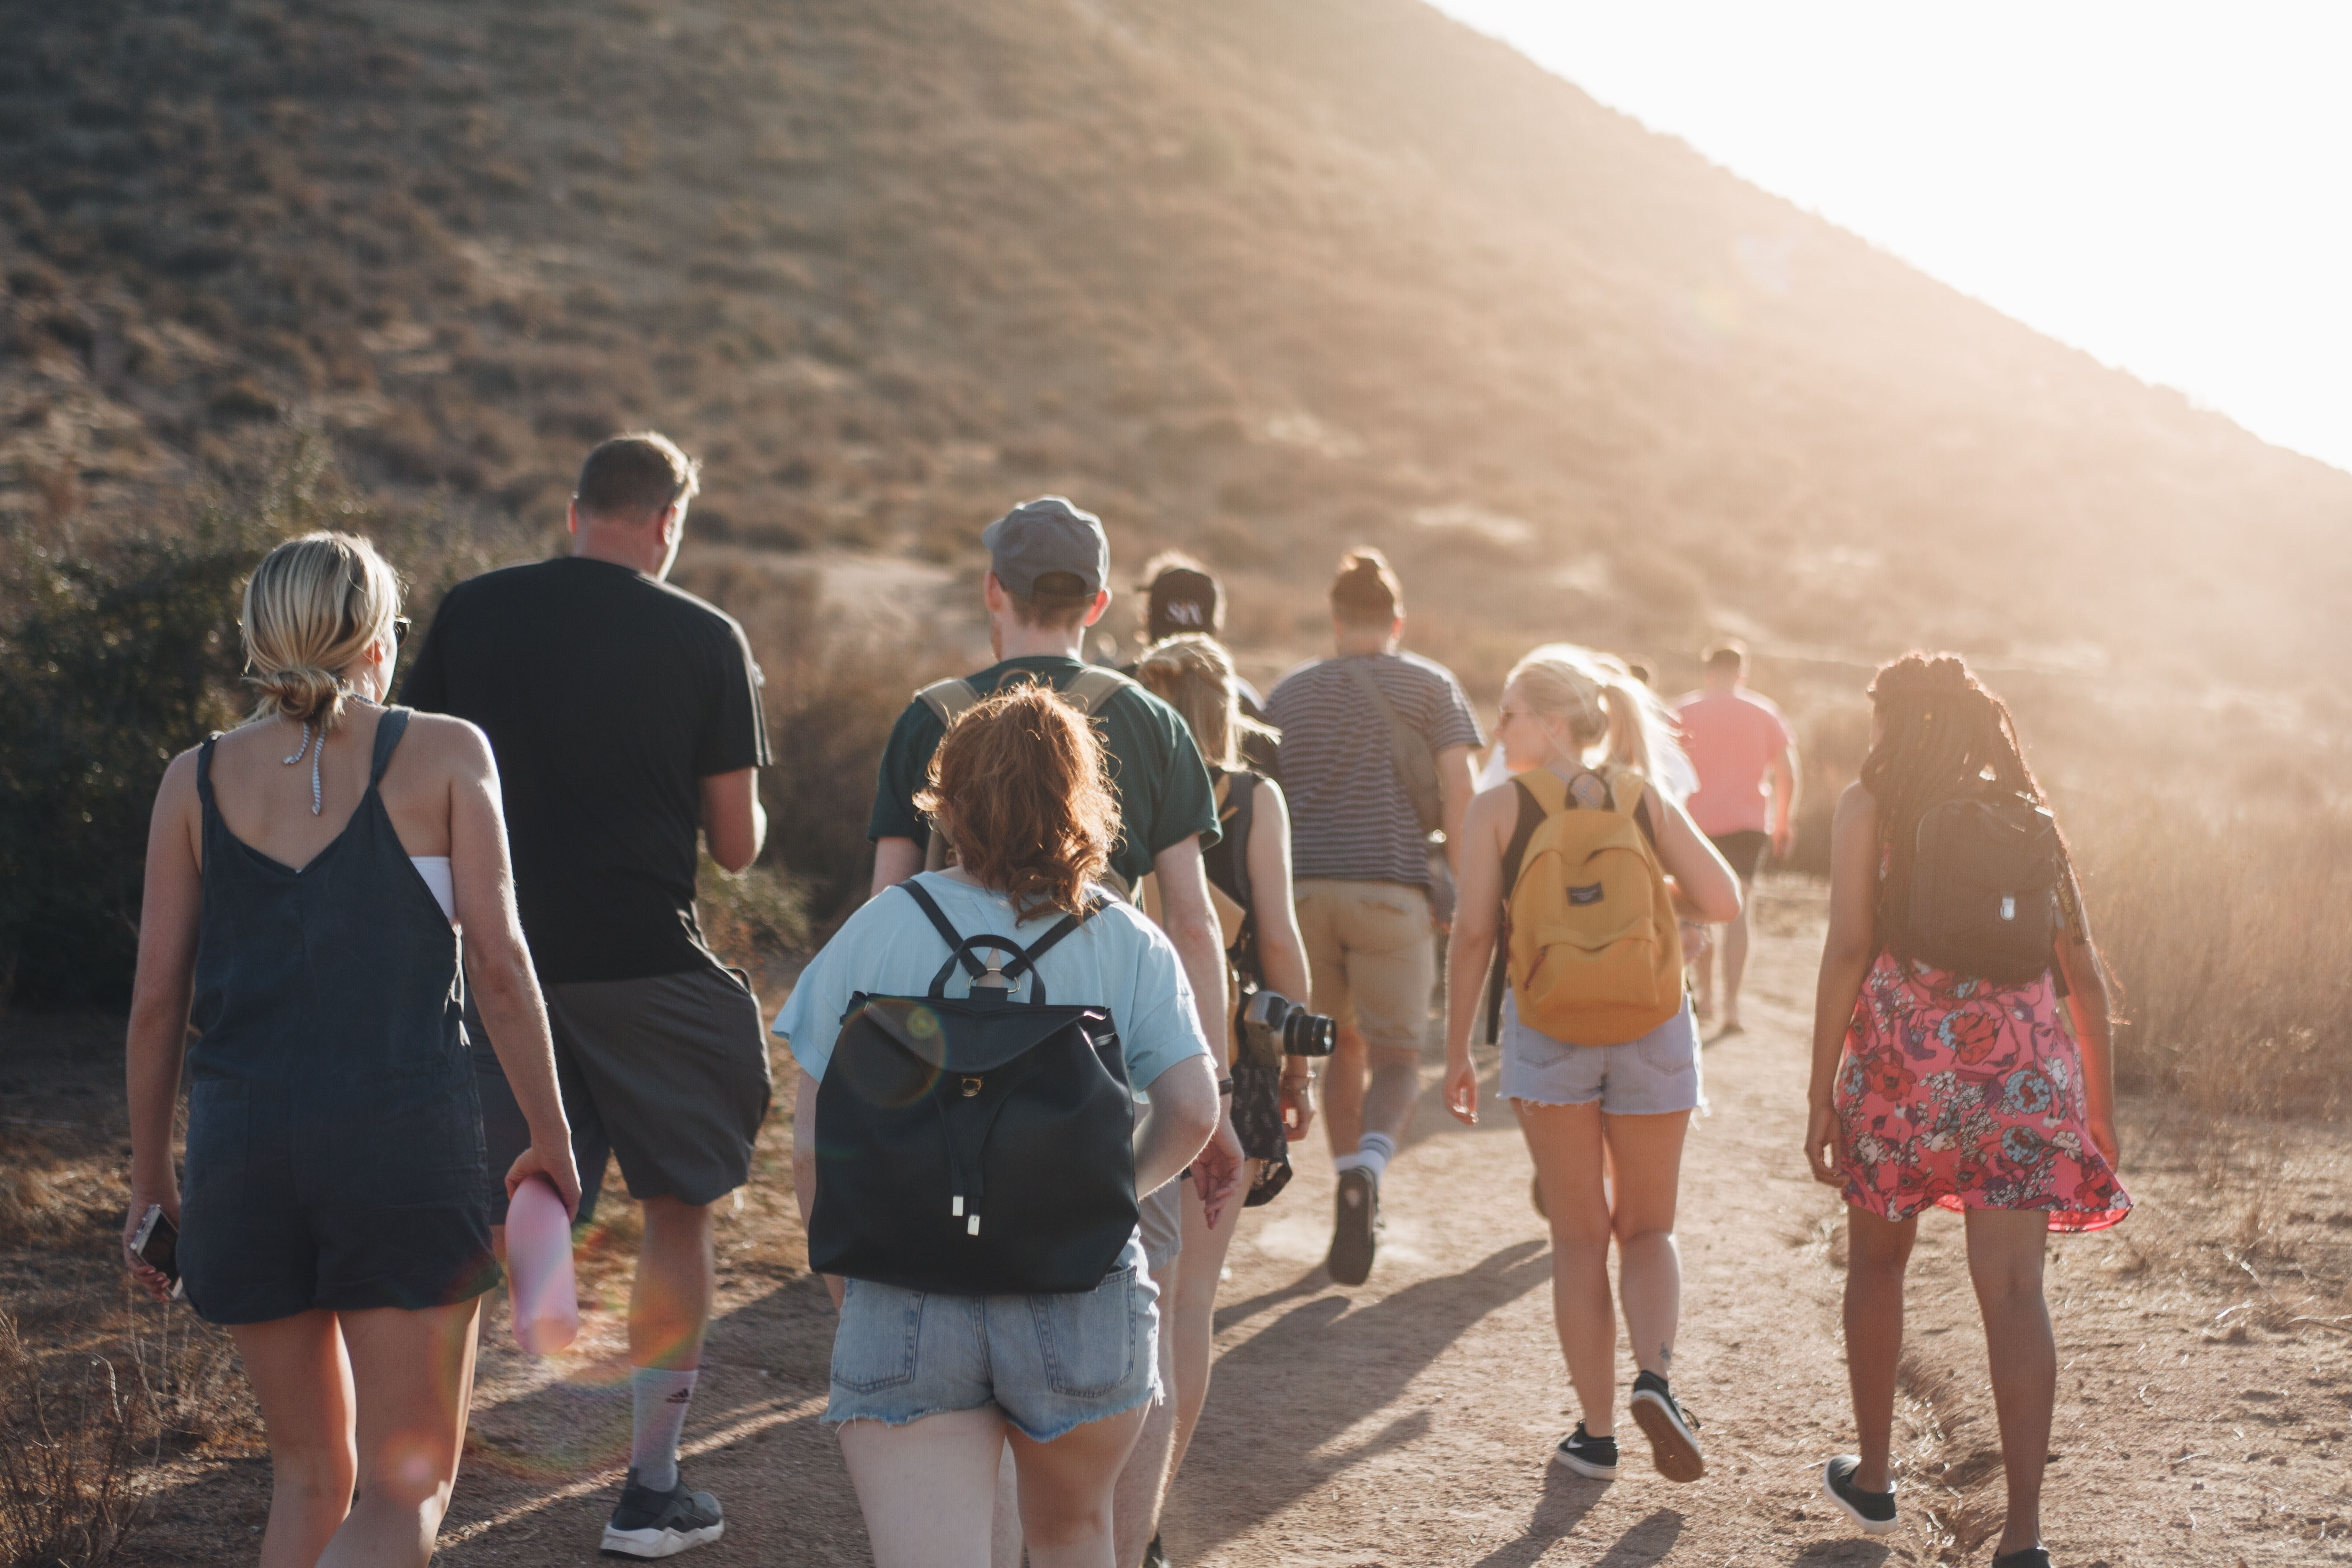
\includegraphics{assets/community/luke-porter-NEqEC7qa9FM-unsplash.jpg}

\hypertarget{title}{%
\chapter{Title}\label{title}}

\hypertarget{title-1}{%
\chapter{Title}\label{title-1}}

\hypertarget{title-2}{%
\chapter{Title}\label{title-2}}

\hypertarget{title-3}{%
\chapter{Title}\label{title-3}}

\hypertarget{title-4}{%
\chapter{Title}\label{title-4}}

\hypertarget{title-5}{%
\chapter{Title}\label{title-5}}

\hypertarget{title-6}{%
\chapter{Title}\label{title-6}}

\hypertarget{title-7}{%
\chapter{Title}\label{title-7}}

\hypertarget{assessment}{%
\chapter*{Assessment}\label{assessment}}
\addcontentsline{toc}{chapter}{Assessment}

The following assignments are opportunities for learners to demonstrate their understanding of the course outcomes. Please confirm assignment details with your instructor, referring to the course syllabus.

Note that Assignment dropboxes are located in Moodle. Also refer to the Course Schedule in Moodle for the specific due dates.

\hypertarget{assignment}{%
\section*{Assignment}\label{assignment}}
\addcontentsline{toc}{section}{Assignment}

\begin{assessment}

\end{assessment}

\hypertarget{grading-criteria}{%
\subsection*{Grading Criteria}\label{grading-criteria}}
\addcontentsline{toc}{subsection}{Grading Criteria}

\hypertarget{references}{%
\chapter*{References}\label{references}}
\addcontentsline{toc}{chapter}{References}

The following are key references used in this course. \textbf{\emph{Check with your course syllabus for required readings.}}

  \bibliography{book.bib}

\end{document}
